\section{1.5 hp Motor}
\subsection{Motor characteristics}

\begin{figure}[htbp]
	\centering
		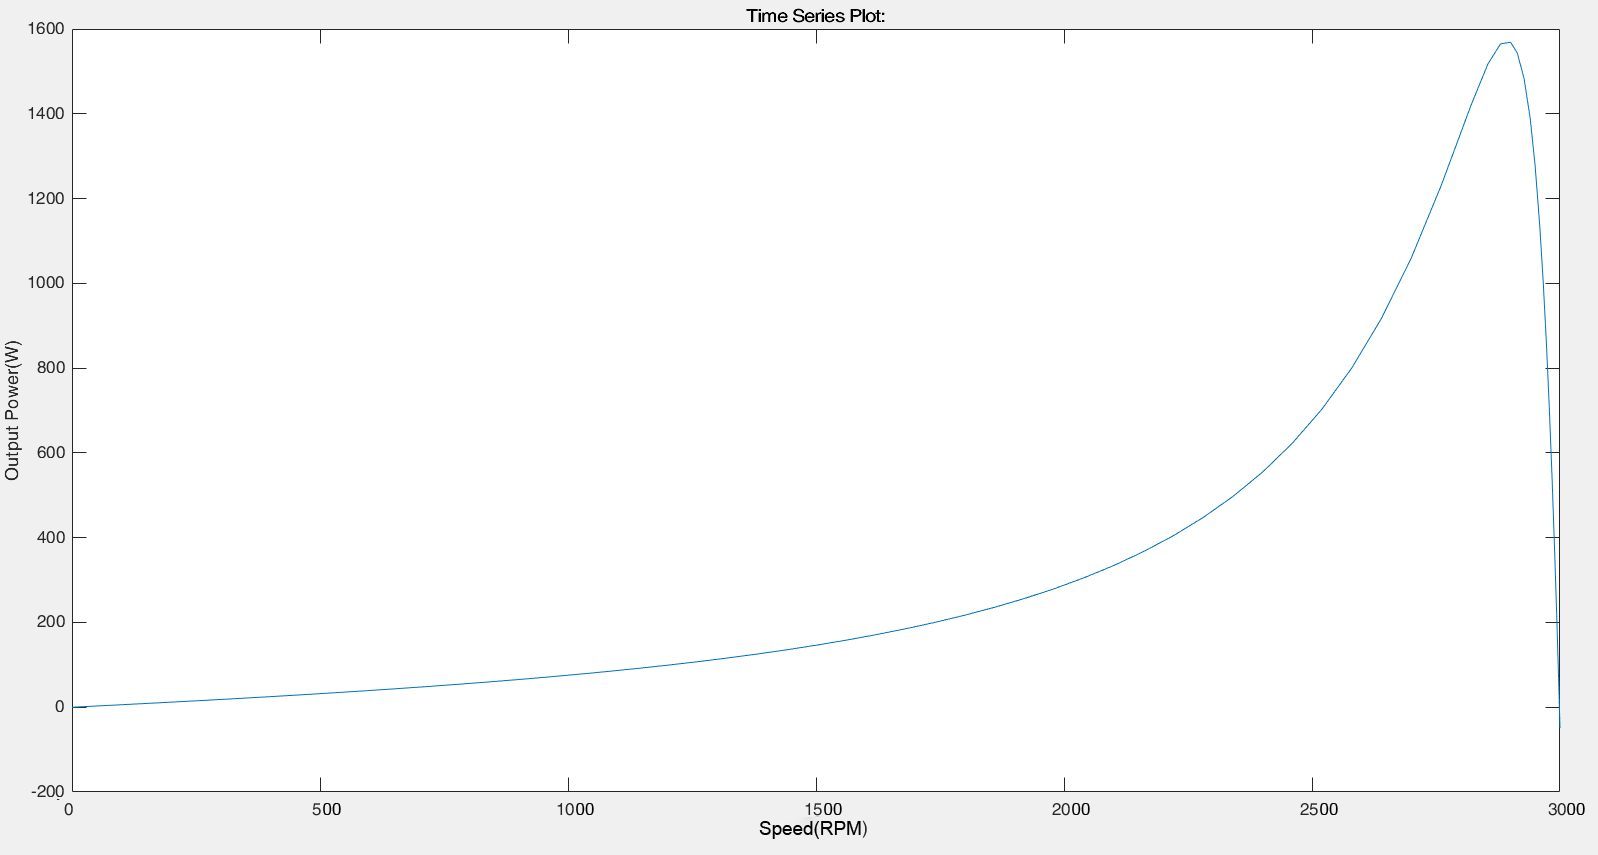
\includegraphics[width = 4.5in]{./Figures/MS/fig512.png}
		\rule{35em}{0.5pt}
	\caption{1.5 hp motor torque-speed characteristics}
	\label{fig:1.5 hp motor torque-speed characteristics} 
\end{figure}

\begin{figure}[htbp]
	\centering
		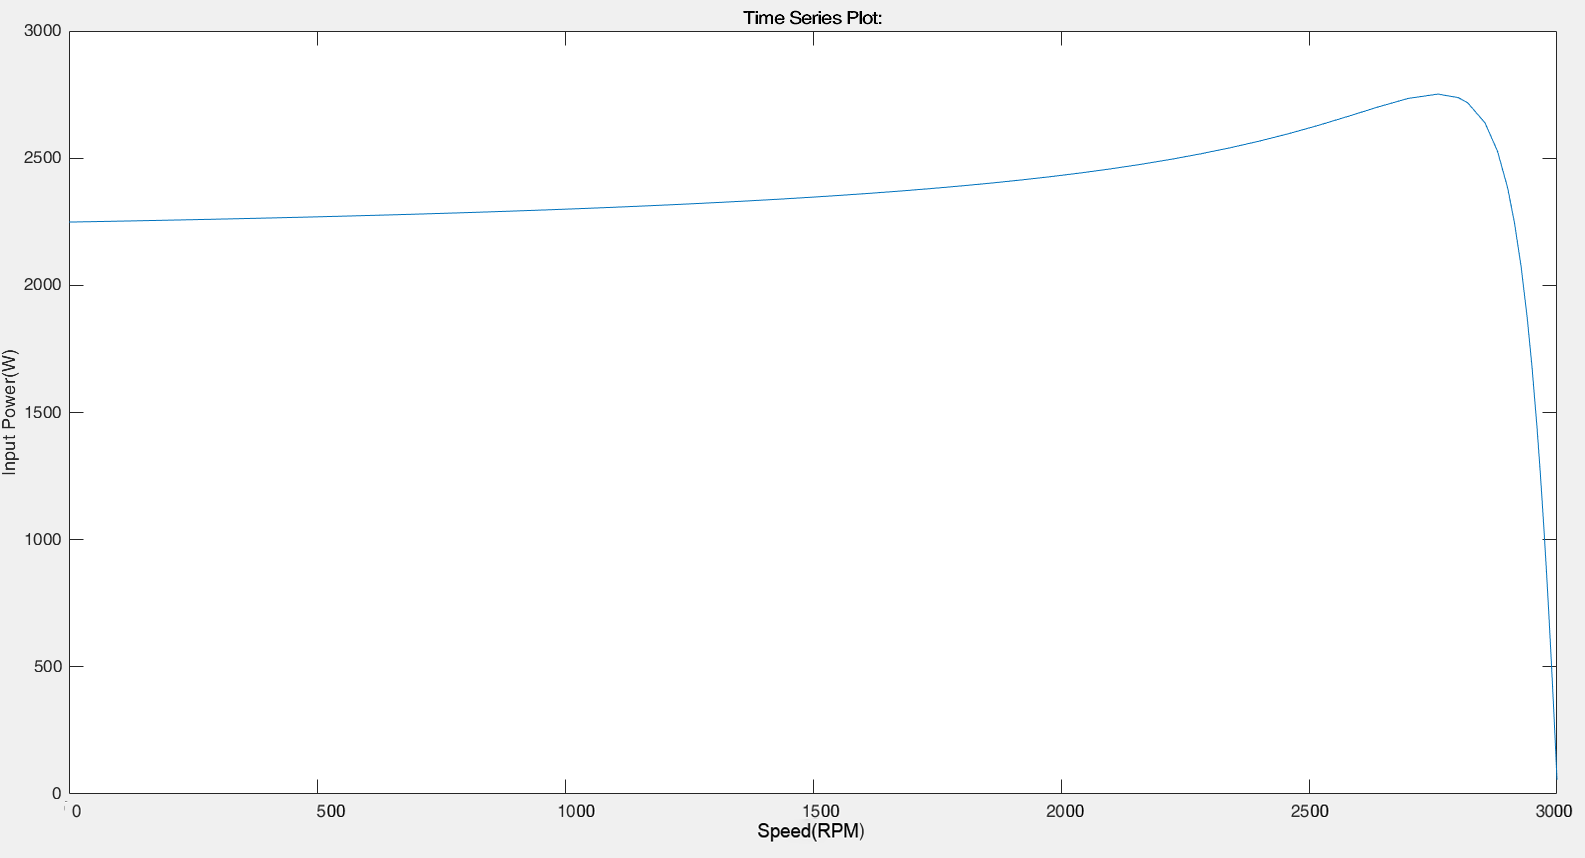
\includegraphics[width = 4.5in]{./Figures/MS/fig513.png}
		\rule{35em}{0.5pt}
	\caption{1.5 hp motor input power characteristics}
	\label{fig:1.5 hp motor input power characteristics} 
\end{figure}

\begin{figure}[htbp]
	\centering
		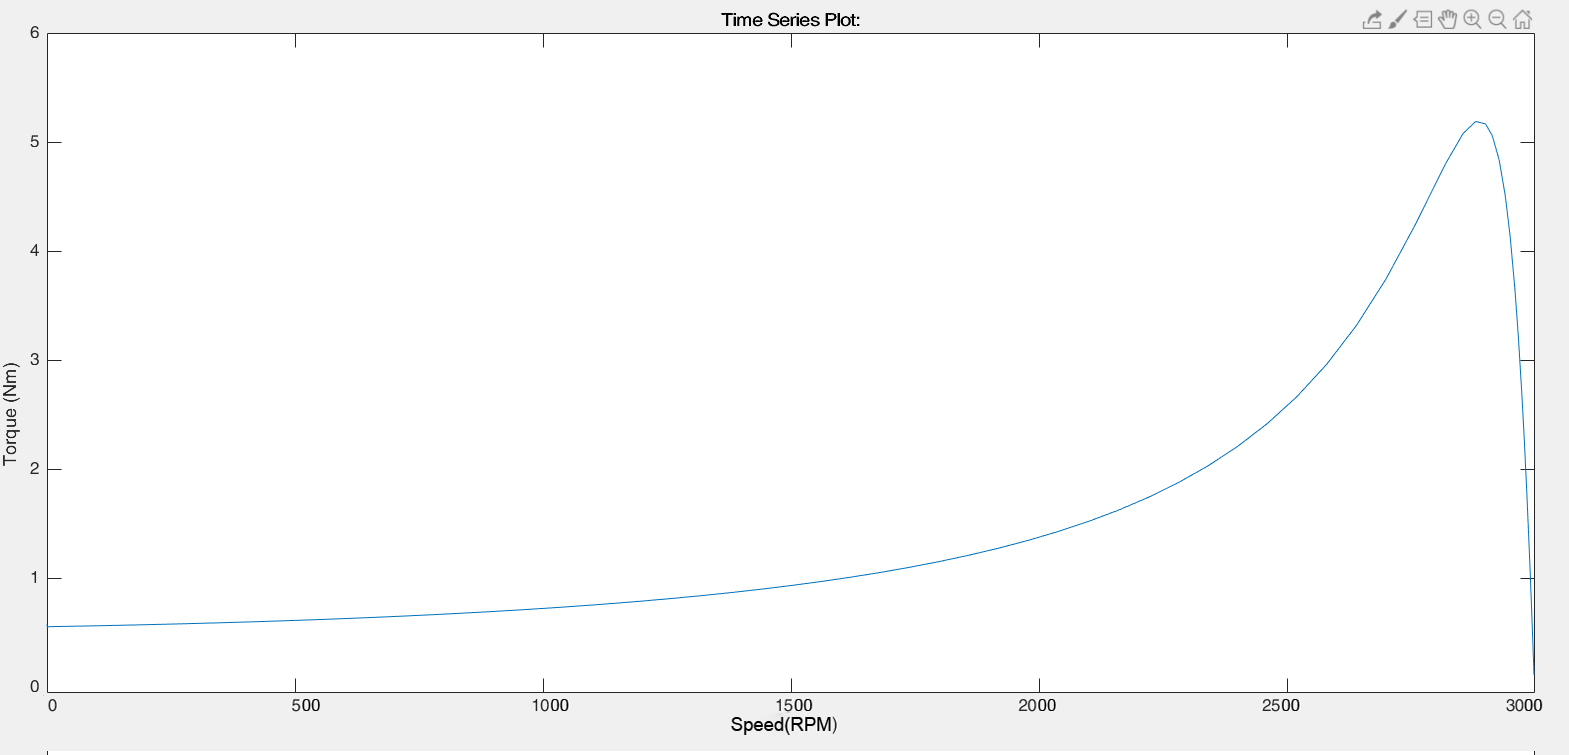
\includegraphics[width = 4.5in]{./Figures/MS/fig514.png}
		\rule{35em}{0.5pt}
	\caption{1.5 hp motor output power characteristics}
	\label{fig:1.5 hp motor output power characteristics} 
\end{figure}

\clearpage
\subsection{Method 1}
\subsubsection{Rated Load Test}
\begin{table}[]
\begin{tabular}{
    >{\columncolor[HTML]{9B9B9B}}l llll}
    \cellcolor[HTML]{656565}{\color[HTML]{000000} Name} & \cellcolor[HTML]{656565}Symbol            & \cellcolor[HTML]{656565}Value     & \cellcolor[HTML]{656565}Unit &  \\
    {\color[HTML]{000000} Current}                      & I                                         & 7.0225                            & A                            &  \\
    {\color[HTML]{000000} Input   Power}                & \cellcolor[HTML]{F2F2F2}P1                & \cellcolor[HTML]{F2F2F2}1473.5    & \cellcolor[HTML]{F2F2F2}W    &  \\
    {\color[HTML]{000000} Speed}                        & w                                         & 309.8536                          & rad/s                        &  \\
    {\color[HTML]{000000} Torque}                       & \cellcolor[HTML]{F2F2F2}T                 & \cellcolor[HTML]{F2F2F2}3.6114    & \cellcolor[HTML]{F2F2F2}Nm   &  \\
    {\color[HTML]{000000} stator   resistance}          & R1                                        & 3.5                               & ohm                          &  \\
    {\color[HTML]{000000} slip}                         & \cellcolor[HTML]{F2F2F2}s                 & \cellcolor[HTML]{F2F2F2}0.0132    & \cellcolor[HTML]{F2F2F2}     &  \\
    {\color[HTML]{000000} Output   Power}               & P2                                        & 1119.00529                        & W                            &  \\
    efficiency                                          & \cellcolor[HTML]{F2F2F2}P2/P1*100         & \cellcolor[HTML]{F2F2F2}75.94199  & \cellcolor[HTML]{F2F2F2}\%   &  \\
    Actual   losses                                     & P1-P2                                     & 354.49471                         & W                            &  \\
    Stator   Copper Loss                                & \cellcolor[HTML]{F2F2F2}Ps                & \cellcolor[HTML]{F2F2F2}172.60427 & \cellcolor[HTML]{F2F2F2}W    &  \\
    Rotor   Copper Loss                                 & Pr                                        & 15.72472                          & W                            &  \\
    Temp   correction factor                            & \cellcolor[HTML]{F2F2F2}k                 & \cellcolor[HTML]{F2F2F2}0.99631   & \cellcolor[HTML]{F2F2F2}     &  \\
    Temp   corrected slip                               & sc                                        & 0.01316                           &                              &  \\
    Temp   corrected Stator copper loss                 & \cellcolor[HTML]{F2F2F2}Ps,c              & \cellcolor[HTML]{F2F2F2}172.60427 & \cellcolor[HTML]{F2F2F2}W    &  \\
    Temp   corrected Rotor copper loss                  & Pr,c                                      & 15.66671                          & W                            &  \\
    Iron Loss                                           & \cellcolor[HTML]{F2F2F2}Pfe               & \cellcolor[HTML]{F2F2F2}95.08894 & \cellcolor[HTML]{F2F2F2}W    &  \\
    Friction\&Windage   Loss                            & Pfw                                       & 29.68700                          & W                            &  \\
    Calculated   Losses                                 & \cellcolor[HTML]{F2F2F2}Ps,c+Pr,c+Pfe+Pfw & \cellcolor[HTML]{F2F2F2}328.04692 & \cellcolor[HTML]{F2F2F2}W    &  \\
    Residual   Losses                                   & P\_Lr                                     & 20.93567                          & W                            & 
\end{tabular}
\end{table}

\subsubsection{Load curve test}
\begin{table}[]
\begin{tabular}{
    >{\columncolor[HTML]{9B9B9B}}l 
    >{\columncolor[HTML]{F2F2F2}}l 
    >{\columncolor[HTML]{F2F2F2}}l 
    >{\columncolor[HTML]{F2F2F2}}l 
    >{\columncolor[HTML]{F2F2F2}}l 
    >{\columncolor[HTML]{F2F2F2}}l 
    >{\columncolor[HTML]{F2F2F2}}l }
    \cellcolor[HTML]{656565}Load   points & \cellcolor[HTML]{656565}125\% & \cellcolor[HTML]{656565}115\% & \cellcolor[HTML]{656565}100\% & \cellcolor[HTML]{656565}75\% & \cellcolor[HTML]{656565}50\% & \cellcolor[HTML]{656565}25\% \\
    Input Power                         & 2052.3                        & 1767.2                        & 1473.5                        & 1087.17                      & 741.54                       & 429.76                       \\
    Current                             & 9.4334                        & 7.9319                        & 7.0225                        & 5.7065                       & 3.7449                       & 2.4687                       \\
    Speed                               & 301.6                         & 305.2435                      & 309.8536                      & 312.4331                     & 313.1374                     & 313.6703                     \\
    Torque                              & 4.637697281                   & 4.215844072                   & 3.6114                        & 2.6862                       & 1.7868                       & 0.8919                       \\
    slip                                & 0.0395                        & 0.0279                        & 0.0132                        & 0.0050                       & 0.0027                       & 0.0011                       \\
    Output Power                        & 1398.7295                     & 1286.8590                     & 1119.0053                     & 839.2578                     & 559.5139                     & 279.7625                     \\
    Actual Losses                       & 653.5705                      & 480.3410                      & 354.4947                      & 247.9122                     & 182.0261                     & 149.9975                     \\
    Efficiency                          & 68.1542                       & 72.8191                       & 75.9420                       & 77.1966                      & 75.4530                      & 65.0974                      \\
    Stator Copper Loss                  & 311.4616                      & 220.2026                      & 172.6043                      & 113.9745                     & 49.0850                      & 21.3307                      \\
    Rotor Copper Loss                   & 64.9914                       & 40.4893                       & 15.9228                       & 4.3819                       & 1.6410                       & 0.3290                       \\
    Calculated Losses                   & 501.2289                      & 385.4679                      & 313.3030                      & 243.1323                     & 175.5020                     & 146.4356                     \\
    P\_lr                               & 152.3416                      & 94.8731                       & 41.1917                       & 4.7799                       & 6.5241                       & 3.5618
\end{tabular}
\end{table}

\subsubsection{No load test}
\begin{table}[]
\begin{tabular}{llll}
    \rowcolor[HTML]{656565} 
    Name                                                              & Symbol  & Value    & Unit  \\
    \cellcolor[HTML]{9B9B9B}Voltage                                   & V\_0    & 220      & V     \\
    \rowcolor[HTML]{F2F2F2} 
    \cellcolor[HTML]{9B9B9B}Current                                   & I\_0    & 2.3112   & A     \\
    \cellcolor[HTML]{9B9B9B}Input   Power                             & P\_0    & 158.4717 & W     \\
    \rowcolor[HTML]{F2F2F2} 
    \cellcolor[HTML]{9B9B9B}Stator   Copper Loss                      & P\_s\_0 & 18.6958  & W     \\
    \cellcolor[HTML]{9B9B9B}Speed at   rated power                    & n\_rl   & 309.8536 & rad/s \\
    \rowcolor[HTML]{F2F2F2} 
    \cellcolor[HTML]{9B9B9B}Torque   Req. to rotate unenergized motor & T\_0    & 0.1858   & Nm    \\
    \cellcolor[HTML]{9B9B9B}Friction\&Windage   Loss                  & P\_fw   & 29.6870  & W     \\
    \rowcolor[HTML]{F2F2F2} 
    \cellcolor[HTML]{9B9B9B}Iron Loss                                 & P\_fe   & 95.0889 & W    
\end{tabular}
\end{table}

\begin{figure}[htbp]
	\centering
		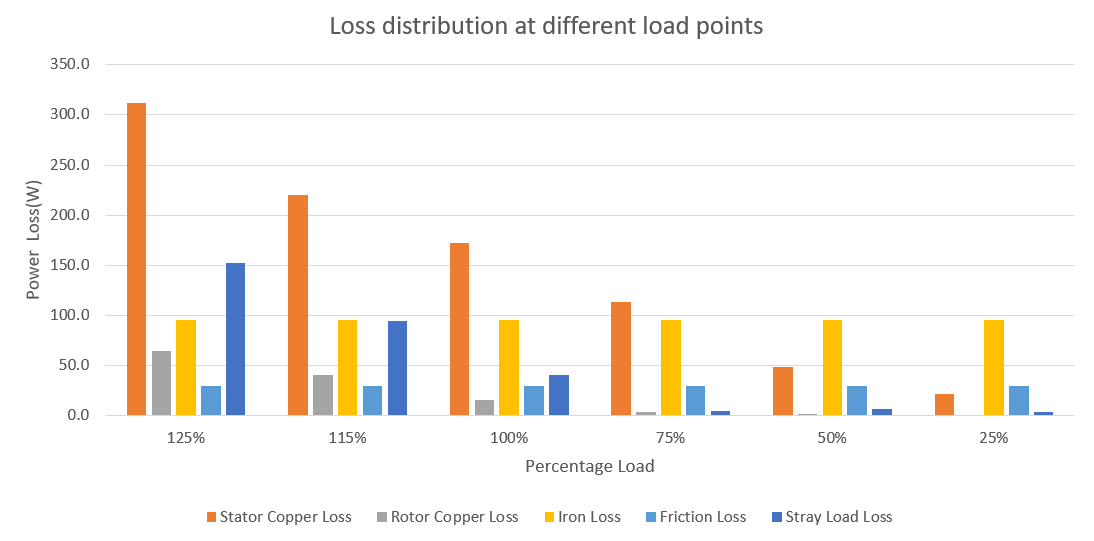
\includegraphics[width = 4.5in]{./Figures/MS/fig515.png}
		\rule{35em}{0.5pt}
	\caption{Bar graph for losses at different load points for 1.5 hp motor(method1)}
	\label{fig:Bar graph for losses at different load points for 1.5 hp motor(method1)} 
\end{figure}
\begin{figure}[htbp]
	\centering
		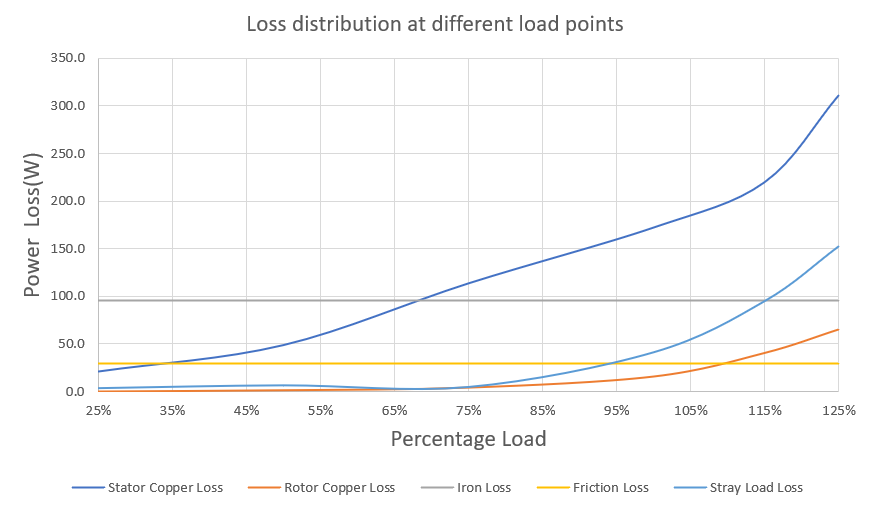
\includegraphics[width = 4.5in]{./Figures/MS/fig516.png}
		\rule{35em}{0.5pt}
	\caption{Line chart for losses at different load points for 1.5 hp motor(method1)}
	\label{fig:Line chart for losses at different load points for 1.5 hp motor(method1)} 
\end{figure}
\begin{figure}[htbp]
	\centering
		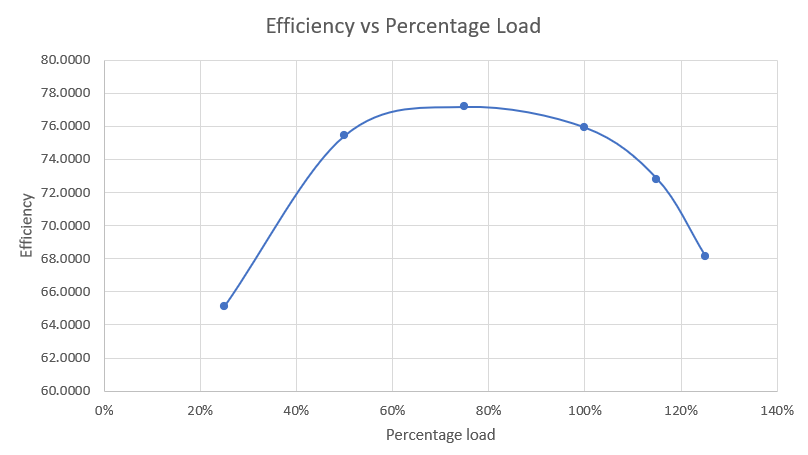
\includegraphics[width = 4.5in]{./Figures/MS/fig517.png}
		\rule{35em}{0.5pt}
	\caption{Percentage load vs efficiency for 1.5 hp motor(method1)}
	\label{fig:Percentage load vs efficiency for 1.5 hp motor(method1)} 
\end{figure}
\begin{figure}[htbp]
	\centering
		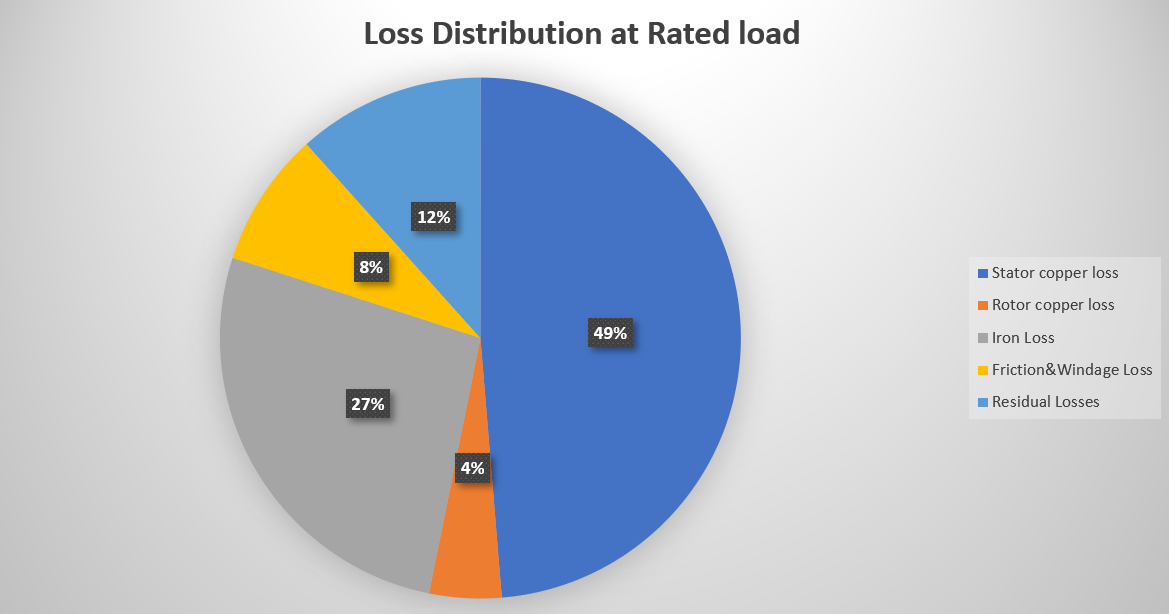
\includegraphics[width = 4.5in]{./Figures/MS/fig518.png}
		\rule{35em}{0.5pt}
	\caption{Pie chart for loss distribution at rated load for 1.5 hp motor(method1)}
	\label{fig:Pie chart for loss distribution at rated load for 1.5 hp motor(method1)} 
\end{figure}

\subsection{Method 2}
\subsubsection{Rated Load Test}
\begin{table}[]
\begin{tabular}{
    >{\columncolor[HTML]{9B9B9B}}l llll}
    \cellcolor[HTML]{656565}{\color[HTML]{000000} Name} & \cellcolor[HTML]{656565}Symbol            & \cellcolor[HTML]{656565}Value     & \cellcolor[HTML]{656565}Unit &  \\
    {\color[HTML]{000000} Current}                      & I                                         & 4.7048                            & A                            &  \\
    {\color[HTML]{000000} Input   Power}                & \cellcolor[HTML]{F2F2F2}P1                & \cellcolor[HTML]{F2F2F2}978.13    & \cellcolor[HTML]{F2F2F2}W    &  \\
    {\color[HTML]{000000} Speed}                        & w                                         & 303.6252                          & rad/s                        &  \\
    {\color[HTML]{000000} Torque}                       & \cellcolor[HTML]{F2F2F2}T                 & \cellcolor[HTML]{F2F2F2}2.4569    & \cellcolor[HTML]{F2F2F2}Nm   &  \\
    {\color[HTML]{000000} stator   resistance}          & R1                                        & 3.9                               & ohm                          &  \\
    {\color[HTML]{000000} slip}                         & \cellcolor[HTML]{F2F2F2}s                 & \cellcolor[HTML]{F2F2F2}0.0330    & \cellcolor[HTML]{F2F2F2}     &  \\
    {\color[HTML]{000000} Output   Power}               & P2                                        & 745.97675                         & W                            &  \\
    efficiency                                          & \cellcolor[HTML]{F2F2F2}P2/P1*100         & \cellcolor[HTML]{F2F2F2}76.26560  & \cellcolor[HTML]{F2F2F2}\%   &  \\
    Actual   losses                                     & P1-P2                                     & 232.15325                         & W                            &  \\
    Stator   Copper Loss                                & \cellcolor[HTML]{F2F2F2}Ps                & \cellcolor[HTML]{F2F2F2}86.32706  & \cellcolor[HTML]{F2F2F2}W    &  \\
    Rotor   Copper Loss                                 & Pr                                        & 26.55133                          & W                            &  \\
    Temp   correction factor                            & \cellcolor[HTML]{F2F2F2}k                 & \cellcolor[HTML]{F2F2F2}0.99631   & \cellcolor[HTML]{F2F2F2}     &  \\
    Temp corrected   slip                               & sc                                        & 0.03292                           &                              &  \\
    Temp   corrected Stator copper loss                 & \cellcolor[HTML]{F2F2F2}Ps,c              & \cellcolor[HTML]{F2F2F2}86.32706  & \cellcolor[HTML]{F2F2F2}W    &  \\
    Temp   corrected Rotor copper loss                  & Pr,c                                      & 26.45339                          & W                            &  \\
    Iron Loss                                           & \cellcolor[HTML]{F2F2F2}Pfe               & \cellcolor[HTML]{F2F2F2}88.20973  & \cellcolor[HTML]{F2F2F2}W    &  \\
    Friction\&Windage   Loss                            & Pfw                                       & 10.22740                          & W                            &  \\
    Calculated   Losses                                 & \cellcolor[HTML]{F2F2F2}Ps,c+Pr,c+Pfe+Pfw & \cellcolor[HTML]{F2F2F2}211.21757 & \cellcolor[HTML]{F2F2F2}W    &  \\
    Residual   Losses                                   & P\_Lr                                     & 20.93567                          & W                            & 
\end{tabular}
\end{table}

\subsubsection{Load curve test}
\begin{table}[]
\begin{tabular}{
    >{\columncolor[HTML]{9B9B9B}}l 
    >{\columncolor[HTML]{F2F2F2}}l 
    >{\columncolor[HTML]{F2F2F2}}l 
    >{\columncolor[HTML]{F2F2F2}}l 
    >{\columncolor[HTML]{F2F2F2}}l 
    >{\columncolor[HTML]{F2F2F2}}l 
    >{\columncolor[HTML]{F2F2F2}}l }
    \cellcolor[HTML]{656565}Load points & \cellcolor[HTML]{656565}125\% & \cellcolor[HTML]{656565}115\% & \cellcolor[HTML]{656565}100\% & \cellcolor[HTML]{656565}75\% & \cellcolor[HTML]{656565}50\% & \cellcolor[HTML]{656565}25\% \\
    Input Power                         & 2051.5                        & 1766.5                        & 1472.4                        & 1086.52                      & 740.89                       & 430.66                       \\
    Current                             & 9.4328                        & 7.9311                        & 7.0218                        & 5.7034                       & 3.7456                       & 2.4664                       \\
    Speed                               & 301.8                         & 305.2142                      & 309.8572                      & 312.4219                     & 313.1297                     & 313.6544                     \\
    Torque                              & 4.634621272                   & 4.216291378                   & 3.6111                        & 2.686156124                  & 1.78686                      & 0.889113                     \\
    slip                                & 0.0389                        & 0.0280                        & 0.0132                        & 0.0050                       & 0.0028                       & 0.0011                       \\
    Output Power                        & 1398.7287                     & 1286.8720                     & 1118.9253                     & 839.2140                     & 559.5189                     & 278.8743                     \\
    Actual Losses                       & 652.7713                      & 479.6280                      & 353.4747                      & 247.3060                     & 181.3711                     & 151.7857                     \\
    Efficiency                          & 68.1808                       & 72.8487                       & 75.9933                       & 77.2387                      & 75.5198                      & 64.7551                      \\
    Stator Copper Loss                  & 311.4220                      & 220.1582                      & 172.5699                      & 113.8507                     & 49.1033                      & 21.2910                      \\
    Rotor Copper Loss                   & 63.9136                       & 40.6064                       & 15.8949                       & 4.4105                       & 1.6538                       & 0.3459                       \\
    Calculated Losses                   & 500.1115                      & 385.5406                      & 313.2407                      & 243.0372                     & 175.5331                     & 146.4128                     \\
    P\_lr                               & 152.6598                      & 94.0874                       & 40.2340                       & 4.2688                       & 5.8380                       & 5.3729\end{tabular}
\end{tabular}
\end{table}

\subsubsection{No load test}
\begin{table}[]
\begin{tabular}{llll}
    \rowcolor[HTML]{656565} 
    Name                                                              & Symbol  & Value    & Unit  \\
    \cellcolor[HTML]{656565}Voltage                                 & V\_0    & 220      & V       \\
    \rowcolor[HTML]{F2F2F2} 
    \cellcolor[HTML]{656565}Current                                 & I\_0    & 1.5107   & A       \\
    \cellcolor[HTML]{656565}Input Power                             & P\_0    & 106.4249 & W       \\
    \rowcolor[HTML]{F2F2F2} 
    \cellcolor[HTML]{656565}Stator Copper Loss                      & P\_s\_0 & 7.9877   & W       \\
    \cellcolor[HTML]{656565}Speed at rated power                    & n\_rl   & 303.6252 & rad/s   \\
    \rowcolor[HTML]{F2F2F2} 
    \cellcolor[HTML]{656565}Torque Req. to rotate unenergized motor & T\_0    & 0.0307   & Nm      \\
    \cellcolor[HTML]{656565}Friction\&Windage Loss                  & P\_fw   & 10.2274  & W       \\
    \rowcolor[HTML]{F2F2F2} 
    \cellcolor[HTML]{656565}Iron Loss                               & P\_fe   & 88.2097  & W      
\end{tabular}
\end{table}
\begin{figure}[htbp]
	\centering
		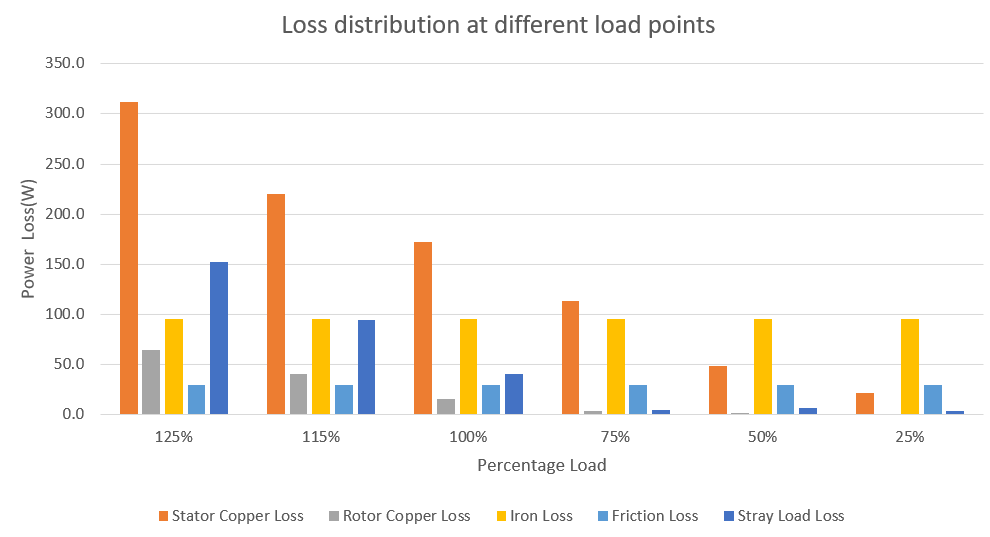
\includegraphics[width = 4.5in]{./Figures/MS/fig519.png}
		\rule{35em}{0.5pt}
	\caption{Bar graph for losses at different load points for 1.5 hp motor(method2)}
	\label{fig:Bar graph for losses at different load points for 1.5 hp motor(method2)} 
\end{figure}
\begin{figure}[htbp]
	\centering
		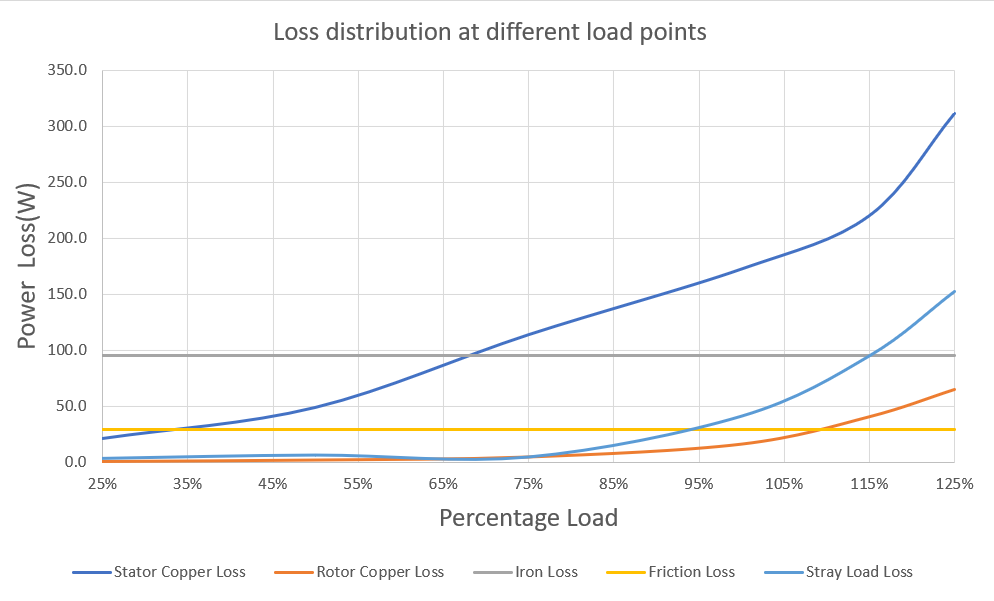
\includegraphics[width = 4.5in]{./Figures/MS/fig520.png}
		\rule{35em}{0.5pt}
	\caption{Line chart for losses at different load points for 1.5 hp motor(method2)}
	\label{fig:Line chart for losses at different load points for 1.5 hp motor(method2)} 
\end{figure}
\begin{figure}[htbp]
	\centering
		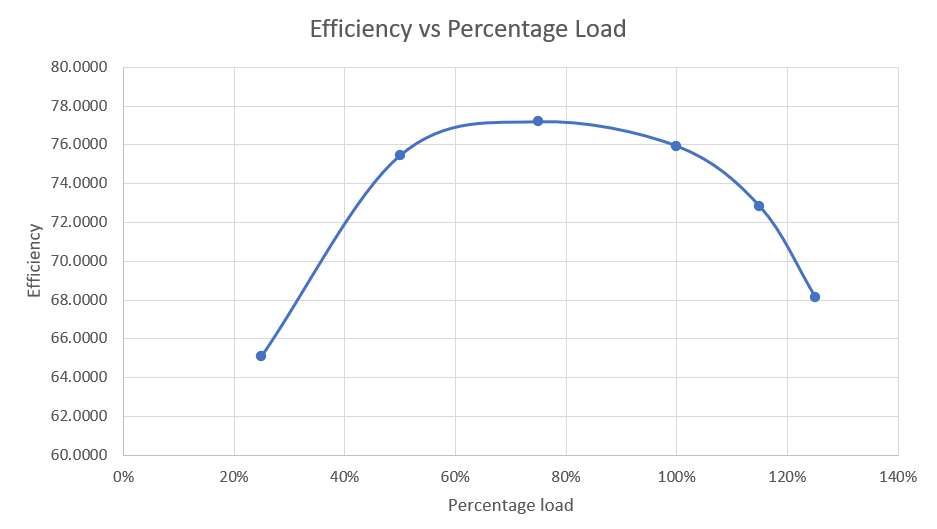
\includegraphics[width = 4.5in]{./Figures/MS/fig521.png}
		\rule{35em}{0.5pt}
	\caption{Percentage load vs efficiency for 1.5 hp motor(method2)}
	\label{fig:Percentage load vs efficiency for 1.5 hp motor(method2)} 
\end{figure}
\begin{figure}[htbp]
	\centering
		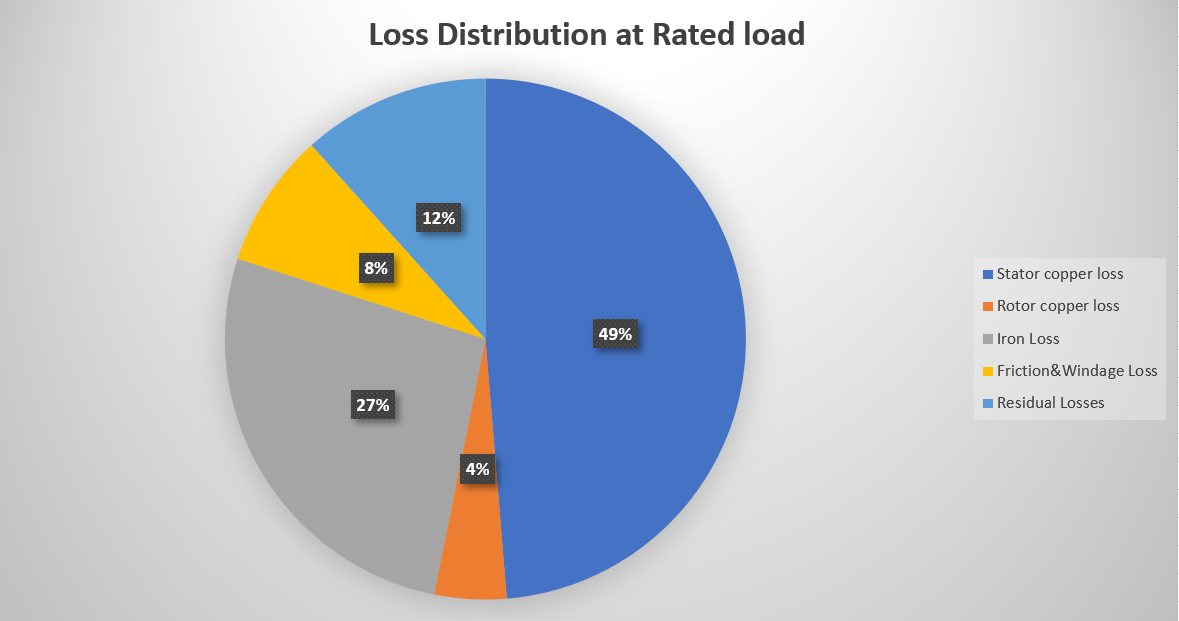
\includegraphics[width = 4.5in]{./Figures/MS/fig522.png}
		\rule{35em}{0.5pt}
	\caption{Pie chart for loss distribution at rated load for 1.5 hp motor(method2)}
	\label{fig:Pie chart for loss distribution at rated load for 1.5 hp motor(method2)} 
\end{figure}